\documentclass[titlepage, a4paper, 11pt]{scrartcl}

%too much whitespace otherwise
\usepackage[left=35mm,top=26mm,right=26mm,bottom=15mm]{geometry}

% deutsche Übersetzungen
%\usepackage[ngerman]{babel}
% Grafik Pakete
\usepackage{graphicx,hyperref,amssymb}
% Ordner für Grafiken
\graphicspath{ {./images/} }
% Pakete für Formatierung der Grafiken
\usepackage{wrapfig}
\usepackage{float}
% deutsches Encoding (Umlaute)
\usepackage[utf8]{inputenc}
% für Grad Symbol
\usepackage{textcomp}


%image grid
\usepackage{graphicx}
\usepackage{subfig}

%\usepackage{multicol}

% Header and Footer
\usepackage{fancyhdr}


\pagestyle{fancy}
\fancyhf{}
\rhead{Lückert, Neudecker}
\lhead{Kalman-filter for partial linear systems for tracking of pool balls}
 
\begin{document}

    \title{Kalman-filter for partial linear systems for tracking pool balls}
    \author{Marlon Lückert \\ Bachelor of Science \\ \href{mailto:marlon.lueckert@haw-hamburg.de}{marlon.lueckert@haw-hamburg.de} 
    \and Julius Neudecker \\ Bachelor of Science \\ \href{mailto:julius.neudecker@haw-hamburg.de}{julius.neudecker@haw-hamburg.de} }
    \date{June 2020}
    \maketitle

    \tableofcontents

    \begin{abstract}
        In this document we are going to discuss an advanced implementation of the Kalman-filter \cite{kalman} improve measurement quality and predict the movement of balls on a pool table. 
        We are going to point out the necessity of an advanced filter design in this particular case. The Problem we are going to solve is the following:
        Since the performance of the filter deteriorates in cases of a rapid change in direction, the filter has to be able to adapt more quickly to these rapid changes.
        Our plan is to derive an implementations with adaptive behavior. The implementation will be tested in a simulator and with real world video footage of a pool table.
        The goal is to provide a filter design with a significant lower MSE than a vanilla implementation. Furthermore we will point out our methods of research, literature sources
        and provide a deep insight in our data analyzation.
    \end{abstract}


    \section{Introduction}
    At first glance the game of pool is very suitable to examine the behavior of a kalman-filter enhanced tracking system based on pure visual tracking. 
    The surface of a pool table is made of a thin fabric which covers a hard surface i.e. slate or granite.
    The balls nowadays are usually made out of resin. This combination of materials creates very small rolling resistance and the balls behave almost fully elastic on collision.
    Since this is only a 2 DOF\footnote{Dimensions Of Freedom - determines the possible rotation or translation along each given axis} problem, this can be solved with a simple linear kalman filter implementation. 
    The problem is, when two balls hit each other or a cushion the velocity vector changes its orientation instantly. 
    If this isn't taken into account, the filter needs some time to adapt to the new direction of movement and will produce wrong estimations during this time.

    This behavior is independent of the type of kalman implementation being constant-velocity-model or constant-acceleration-model.
    A kalman filter will assume the direction of movement on any given sample is about the same as in the last sample. 
    It will therefore create wrong estimations if the direction of movement changes drastically in a short period of time. The time the filter needs to recover depends on the filter gain.

    We also use the filter to predict values for any given length into the future by feeding back its estimations as actual state. 
    The quality of this prediction however depends on several factors, i.e. the applied process noise and framerate of the video.

    \section{Problem and Motivation}
    As introduced in the previous section is the lack of adaptability in a vanilla Kalman implementation.
    One could argue that this can be taken into account by using a higher overall process noise which would in turn lead to significantly reduced overall quality.
    This gets worse with increased speed and lower framerate. Essentially rendering the filter useless at a certain point.

    We think this is a good point to develop this algorithm for future application in VR and AR based pool trainers and augmented broadcast experiences.

    \section{Hypothesis and Goals}

    We can improve the algorithm in the Kalman-Filter by taking the environment into account.
    If we feed the algorithm with the position of objects which could cause a collision,
    the filter can dynamically react to those sudden changes in the direction of movement.

    \section{State of research}

    Jong-Yun Kim and Tae-Yong Kim \cite{kim} developed a method to provide robust tracking of a soccer ball. 
    They provide a solution for the problem for the case that the soccer ball might be occluded by the player at any given time,
    which results in a diminished tracking accuracy. 
    In this case they used the velocity vector of the player to substitute for the ball presuming that the ball moves in the same direction as the player does.

    Jia et.al. \cite{jia} conducted research in the trajectory of pool balls, which helped us to decide which kalman model is the most suitable.

    Shiuh et.al. \cite{shiuh} provided a good starting point how to create a tracking algorithm for pool balls. They also developed an algorithm to track occluded objects using an adaptive kalman filter.
    In this case they used to threshold in order to determine whether the object can still be reliably tracked. If this isn't the case the filter will rely only on predicted values until the object can be tracked reliably again.

    Salzmann and Urtasun \cite{salzmann} proposed a more general approach for tracking. 
    They were able to recreate a highly accurate tracking from a noisy picture based on newtons 2nd law and markov models.
    Using different constraints and presumptions they were even able to extract physical parameters like friction and trajectories.

    Mohamed and Schwarz \cite{schwarz} are using partly the same approach as we do to improve the results created by INS/GPS\footnote{Inertial Navigation System / Global Positioning System} Systems.
    However their approach only targets the 'Q' and 'R' parameters of the filter.

    Sarkka and Nummenmaa \cite{sarkka} created an adaptive kalman implementation which adapts itself to time-varying noise parameters. Since our input data is constant in this regard,
    we decided to simulate for the optimal filter parametrization instead of relying on the filter to adapt itself.

    Gabdulkhakova and Kropatsch \cite{kropatsch} use a kalman filter to create a video analysis tool for snooker game broadcasting.

    \section{Methods of research}

    We are going to use two stepped approach: develop and the algorithm in a tailor made simulation
    and evaluate the results with real footage video. Our main instrument of validation will be the MSE
    \footnote{Mean Square Error} between the ground truth and filtered position and the quality of prediction
    with +n frames respectively.

    We are going to use a two-stepped approach: 
    
    Firstly we will optimize the process noise behaviour in edge cases. 
    Meaning that at points where the ball is at risk of a sudden change in direction, the filter adapts itself by temporarily altering its process noise parameter.
    Thus being less prone to overshooting the critical point.
    We are planning to use a gradient descent algorithm in order to optimize the filter behavior in all states.

    Secondly since a rapid change in direction is not a linear problem in terms of implementation of a kalman filter, we are plannning on using linear algebra to reduce this problem 
    to a linear vector multiplication. By doing so we will achieve not only a sudden but also precise change without utilizing the time invariant input capabilities of the filter.

    \section{Research Goals}

    Primarily we are looking for related work in the field of kalman filtering in billiards, to inform ourselves about the current progress of research and state-of-the-art solutions.

    Secondly our goal with the literature research is to find sources of information which complements our expertise. 

    While writing our proposal we identified five aspects where we lack sufficient expertise.
    These are in particular:

        \paragraph{Design of experiments}

        As outlined in the research proposal we are going to develop our ideas in a simulation. Therefore it is efficient to design the experimental part in advance.
        This means that we are not going to use a trial-and-error approach but instead invest some time to think about possible outcomes and how to achieve these by 
        altering different parameters in particular and develop a deeper understanding of their behavior.

        \paragraph{Gradient descent algorithms}

        Since there exist a huge number of different numerical and analytical ways to solve a gradient descent problem it will save time to evaluate the best
        suitable algorithm prior to implementation to avoid unnecessary work.

        \paragraph{Efficient implementation of algorithms}

        This is especially important since our algorithm is supposed to work in realtime.
        Therefore any delay induced by inefficient code is unacceptable.

        \paragraph{openCV best practices}

        The analysis of the original footage is made by openCV. Since this library offers a wide variety of different approaches to isolate objecs in videofootage,
        it is evaluate the best option.

        \paragraph{Measure and comparison of quantifiable data}

        The results in our research will be mainly represented by numbers. To create a better understanding of these numbers and how they interact it is a good approach to 
        evaluate different methods of putting numbers in context to one another and which scales and graphs are the quasi standard across the research community.


    \section{Source of Information}

    For the research regarding \textit{state-of-the-art solutions} and \textit{efficient implementation of algorithms and openCV best practices} it is the best option to look for recent papers since these topics are currently
    subjects where a certain number of people are working on. Therefore the following archives offer a good starting point to search for up-to-date papers:

    \begin{enumerate}
        \item IEEE online database
        \item arXiv.org
        \item ACM Digital Library
        \item Google Scholar
    \end{enumerate}

    The Topics \textit{statistical experimental design and measure and comparison of quantifiable data} are already established in the scientific community.
    Therefore it is the best approach to consult the latest literature in these particular fields. In our case this can be done to a certain extent with the HIBS database
    and online services or with actual books in the library.

    \textit{The efficient implementation of algorithms} is less of a scientific problem but of a code-optimization. Hence reading blogs of skilled programmers or threads on
    \textit{Stackoverflow} seems as the most reasonable approach.

    \section{Criteria for eligible sources}

    The general criteria for any sources are mostly common sense:

    \begin{itemize}
        \item credibility and plausibility
        \item a certain standard of quality
        \item integrity
    \end{itemize}

    These criteria might seem overly cautious in case the source is a book written by any member of the scientific community. However in the case of short paper or online blog
    the author of that particular source might not be as credible. Therefore a higher level of scrutiny with the informations provided is necessary.

    Furthermore since the sources might be cited in a paper or dissertation they have to be scientificly quotable. This is expecially true to protect the resulting work against 
    accusations of plagiarism.

    As already pointed out in the previous section some topics are more subject to change due to present research activities
    and must therefore reflect the most recent state of research. 

    Another important aspect is especially the case with non-scientific online ressources as blogs and the previously mentioned
    \textit{Stackoverflow}. Since these sources are also subject to change, it is important to keep track of the particular
    version of the ressource to prevent confusion in case the ressources changes.

    \section{Sources for our research}

        \subsection{Related Work}

        Jong-Yun Kim and Tae-Yong Kim \cite{kim} developed a method to provide robust tracking of a soccer ball. 
        They provide a solution for the problem for the case that the soccer ball might be occluded by the player at any given time,
        which results in a diminished tracking accuracy. 
        In this case they used the velocity vector of the player to substitute for the ball presuming that the ball moves in the same direction as the player does.

        Jia et.al. \cite{jia} conducted research in the trajectory of pool balls, which helped us to decide which kalman model is the most suitable.

        Shiuh et.al. \cite{shiuh} provided a good starting point how to create a tracking algorithm for pool balls. They also developed an algorithm to track occluded objects using an adaptive kalman filter.
        In this case they used to threshold in order to determine whether the object can still be reliably tracked. If this isn't the case the filter will rely only on predicted values until the object can be tracked reliably again.

        Salzmann and Urtasun \cite{salzmann} proposed a more general approach for tracking. 
        They were able to recreate a highly accurate tracking from a noisy picture based on newtons 2nd law and markov models.
        Using different constraints and presumptions they were even able to extract physical parameters like friction and trajectories.

        Mohamed and Schwarz \cite{schwarz} are using partly the same approach as we do to improve the results created by INS/GPS\footnote{Inertial Navigation System / Global Positioning System} Systems.
        However their approach only targets the 'Q' and 'R' parameters of the filter.

        Sarkka and Nummenmaa \cite{sarkka} created an adaptive kalman implementation which adapts itself to time-varying noise parameters. Since our input data is constant in this regard,
        we decided to simulate for the optimal filter parametrization instead of relying on the filter to adapt itself.

        Gabdulkhakova and Kropatsch \cite{kropatsch} use a kalman filter to create a video analysis tool for snooker game broadcasting.

        In the article \cite{wu2017capturing} they use a Kalman filter for smooth estimations of a billiards game.

        In \cite{8273755} they present an adaptive kalman filter, which estimates Q and R values. 

        \subsection{Design of experiments}

        To get a general sense of how statistical experimental design works these Books provide a good introduction into this topic: \cite{siebertz2017statistische} and \cite{retzlaff1978statistische}.
        Both books are available at our local Library.

        A more practical approach is outlined in the articles \cite{hoevelmann1993statistische} and \cite{schweitzer1992off}.

        \cite{siebertz2017doe} is a good source of examples to put everything in context.

        \subsection{Gradient  descent  algorithms}

        Although the gradient descent method is often used in Machine Learning to optimize parameters in neural networks, we can use it to solve our optimization problem.
        The articles \cite{ketkar2017deep} and \cite{marti2005stochastic} provides an introduction to the optimization problem with GD methods whereas \cite{marti2005stochastic} gives an overview with more advanced methods.

        \cite{bishop2006pattern} is a very famous book for more advanced topics. Since we've got a basic understanding of how to implement GD in our simulation, we might consider using 
        some advanced techniques from this book. This might prove especially useful because the normal gradient descent method can only find local minimas.

        \subsection{Efficient implementation  of  algorithms}

        There exist a few different approaches to optimize an algorithm for fast execution. These are in particular paralelization and compiletime optimization.

        Since our optimized filter will highly rely on vector and matrix operations, there is a big potencial for all these optimizations. However since we lack experience in
        writing special code like this, we have to make us familiar with the basics of such coding.

        For paralelization through parallel hardware we could use openCL. An comprehensive introduction is provided by \cite{trevett2013opencl} and \cite{tompson2012introduction}.
        Depending on the hardware we also might go with a proprietary GPGPU framework such as CUDA. In case we should decide to use this \cite{nickolls2008scalable} is an introduction into this topic.

        An introduction in compiletime optimization is provided by \cite{hohenauer2006retargetable} and introduction on how to use the new AVX instruction on Intel Processors is given by \cite{cornea2015intel}.

        \subsection{openCV best practices}

        With the article \cite{janku2016comparison} we can get an overview and comparison of different detection algorithms for the OpenCV framework.

        The article \cite{gao2018design} gives an insight on how to design a multi-object detection system for billiards in openCV, which perfectly fits our research case.

        The conference paper \cite{gabel2018jetson} uses neural networks in conjunction with openCV to detect balls.
        This approach aims for an efficient re-training of neural networks. This is useful for our research, because we can easily adopt the algorithm to different pool environments and do not have to manually adjust the ball detection.

        The thesis \cite{schmidt2016measuring} focuses on performance optimization for speed estimation of balls with openCV on mobile devices. This is useful for our research, because we want to achieve real-time tracking and eventually port the application to mobile devices.

        \subsection{Measure and comparison of quantifiable data}

        Because error analysis is the driving factor behind our research since we want to minimize the error which is produced by an inferior filter-design, we have to make ourselves familiar with
        state of the art error analysis and the uncertainties of measurement with \cite{taylor1997introduction}. 

        \cite{allen1971mean} provides a good explanation why in predictions it is better to use the MSE instead of the LSE.

        The standard method to visualize the mean square error of Kalman-filters are 2D plots,
        which can be seen in \cite{8993001} and \cite{1165091}. The y-axis describes the MSE and x-axis the observed parameter.     

    \section{Proposed timetable}

    To conduct our research in a timely manner, we propose the following schedule to have the finished research paper by the end on June 2020.

    \begin{itemize}
        \item until End of June: develop the mathematical framework
        \item until End of July: develop the simulation and create footage for evaluation
        \item until Middle of August: implement the filter according to optimized parameters
        \item until Middle of September: conclude results and write research paper
    \end{itemize}

    We are planning to submit this paper to a conference which has relevance in this particular field of research. This has yet to be determined.


    \section{Operationalization}

    In the following section we are going to operationalize the different terms in our hypthesis.

        \subsection{Tracking}

        The tracking describes the deviation from the filtered position of the billiard ball (result of Kalman-Filter) to the real position of the billiard ball.
        The position divides into three dimensions, the x-coordinate, the y-coordinate, the z-coordinate.
        Since we are investigating a billiard game we disregard the up-direction (z-coordinate), because the ball moves on a flat surface and will not leave the plane.
        We are measuring the coordinates in pixels. The range of the pixels is defined by the resolution of the input video on which the Kalman-Filter gets applied to.
        The origin, coordinate (0,0), is always the top-left corner.
        The final deviation from the two position is calculated with the Euclidean distance, which results in a length in pixels.

        The position of the billiard ball changes over time, because we are investigating video sources.
        To measure the deviation of the whole video and to get a key figure, we are calculating the mean square error (mse) in which the error is the pixel distance between the two positions. 

        \subsection{Prediction}

        The prediction describes the deviation from the calculated future position of the billiard ball to the real position at this specific time.
        The positions use the same measurements as described in the previous chapter.
        The time is measured in frames. The specific number of frames we will look in the future will vary in our experiments.
        To make the frame count comparable with different input video source we align them with the framerate (frames per second) of the video.

        \subsection{Improvement}

        The improvement compares a standard Kalman-Filter to our implementation of the Kalman-Filter.
        The improvement is measured as the difference between the different mean square errors of the tracking and the prediction.
        The smaller the mse of our Kalman-Filter compared to the standard implementation the greater the improvement.

    % \section{Data Acquisition}

    % We are going to acquire our data from billiard simulations and real videos.

    %     \subsection{Simulation}

    %     We construct a simulation to fully control every parameter and the state of the billiard game.
    %     This helps us to accomplish a better conclusion to the performance in real video.
    %     Our examination units are the framerate, the ball velocity, the sensor noise.

    %         \paragraph{Framerate}

    %         The framerate describes the framerate of the video, which is equal to the sampling rate of the Kalman-Filter.
    %         A standard Kalman-Filter performs much worse on low framerate because it gets less data to process.
    %         We test different framerate to inspect the performance of our implementation for different environments.
    %         For realtime applications on mobile devices our implementation has to perform well on low framerates.
    %         We are going to test the standard framerates 30 and 60 FPS and a very low framerate at 10 FPS.

    %         \paragraph{Ball Velocity}

    %         The ball velocity describes the speed of the ball, which depends on how hard the player hits the ball.
    %         The velocity is measured in pixel per frame.
    %         The cover a lot of cases, we choose a low velocity of 300 pixel per frame, an average velocity of 500 pixel per frame and a high velocity of 700 pixel per frame.
    %         We have to keep in mind that a high velocity also leads to more collisions because the ball will move a longer distance.

    %         \paragraph{Sensor Noise}

    %         When we analyze realtime videos we have detect the balls in the video frame.
    %         The detection is not always perfect and heavily relies on the light conditions and resolution of the camera.
    %         To simulate the quality of detection we added a noise value which changes the detected ball position by random value in a certain range.
    %         We test a deviation of 15 pixel, 30 pixel and 60 pixel to inspect how well the Kalman-Filter will perform.

    %         \paragraph{Change of parameters}

    %         To test the parameters individually we only change one parameter at the time.
    %         Three variations on each parameter lead to 9 simulation environments in total.

    %     \subsection{Real Videos}

    %     After testing the filter in the simulation we are also doing some test on random billiard videos.
    %     Since we are relying on a ball detection algorithm to identify the billiard balls, we cannot obtain the real position of the ball like we could in the simulation.
    %     That's why we cannot make statements about the tracking quality, but we can evaluate the performance of the tracking.

    \section{Testing}

    Our Kalman-Filter is specifically designed to track and predict the position of billiard balls.
    The final goal is to implement this filter in a mobile app, which analyzes video footage preferably in realtime.

    To test the filter we compare calculated position of the filter to the real position of the billiard pool.

    But we cannot test our filter with video material because we do not know the ground truth of the balls' position in the video.
    So we are not able to make statements about the quality of the filter if we cannot compare the filter result to the optimal result.

    Therefore we have to develop a virtual test environment where we can control every parameter of the billiard game and know the actual values of the balls' position.

        \subsection{Simulation}

        The simulation has to reflect all characteristics and physical conditions of a real billiard table.
        The virtual environment consists of a billiard ball and four cushions.
        We can control the start acceleration of the ball where we can reflect start shots with different intensity.
        When the ball starts moving a constant deceleration is applied to mimic the friction of the table`s fabric.
        If the ball touches a cushion the direction of movement is mirrored to reflect a collision.

        Our simulation does not include the rotation of the ball which would leads to a different behavior on cushion collisions.
        We have to assume that the ball is hit directly in the middle with no rotation.

        With the simulation we can access all parameter of the ball like the position, speed and acceleration.

        \subsection{Modifying the simulation}

        The purpose of a Kalman-filter is to improve noised sensor data and filter bad measurements.
        When we analyze video footage the ball detection algorithm works as a sensor which provides the estimated position of the ball.
        The quality of this detection depends on different factors like the video resolution or the contrast of the images.
        But the sensor result will never be exactly the ground truth.

        With the simulation we have perfectly correct values. So we have to modify the correct values by adding noise to reflect the real world circumstances.
        We have full control over the amount of noise, which makes it possible to simulate different qualities of sensors.

        The simulation also provides data every time we want them. But in a real example you are limited to the framerate of the video and the performance of the ball detection algorithm.
        Therefore we have to define a sampling rate on which we process the data of the simulation. 

        \subsection{Parameters for testing}

        After we defined the technical frame we can adjust different parameter to modify the simulation.

        \begin{itemize}
            \item start acceleration. How hard is the first hit of the ball?
            \item sensor noise. How close is the estimated position to the real position?
            \item sampling rate. How often is it possible to process a video frame?
        \end{itemize}

        We define three values for each parameter and compare them among each other which results in nine tests.

        For the start acceleration we choose a slow hit with 80 cm/s, a medium hit with 1 m/s and a power shot with 4 m/s \cite{ballspeed}

        For the sensor noise we choose a deviation of 10 pixels, 50 pixels and 100 pixels.

        For the sampling rate we choose 15 fps (very slow algorithm), 30 fps (realtime on typical mobile devices), 60 fps (realtime on modern devices).

        Each of the nine tests are run with the standardized Kalman-filter and our filter implementation.

        \subsection{Data acquisition}

        With each test run we collect the estimated position with the normal Kalman-filter, our implementation and the ground truth.
        Additionally to the current position we collect the prediction of the position in 0.2 seconds, 1 second and 2 seconds.

    \section{Evaluation}

    In order to evaluate if and how much better our filter implementation performs compared to the standardized Kalman-Filter
    we run the previous described tests and compare the results.

    The key figure of evaluation is the mean square error.
    If the mean square error of our implementation is lower compared to the standard implementation in every experiment 
    we can prove that our implementation improved the tracking and prediction of billiard balls.

    Since we are running multiple test with different parameters we can make statements about what parameter has the biggest influence of the quality of the filter. 
    The outcome of these evaluations might for example look like the following, where we compare the actual position and its prediction of the different implementations:

    \begin{figure}[H]
        \centering
        \fbox{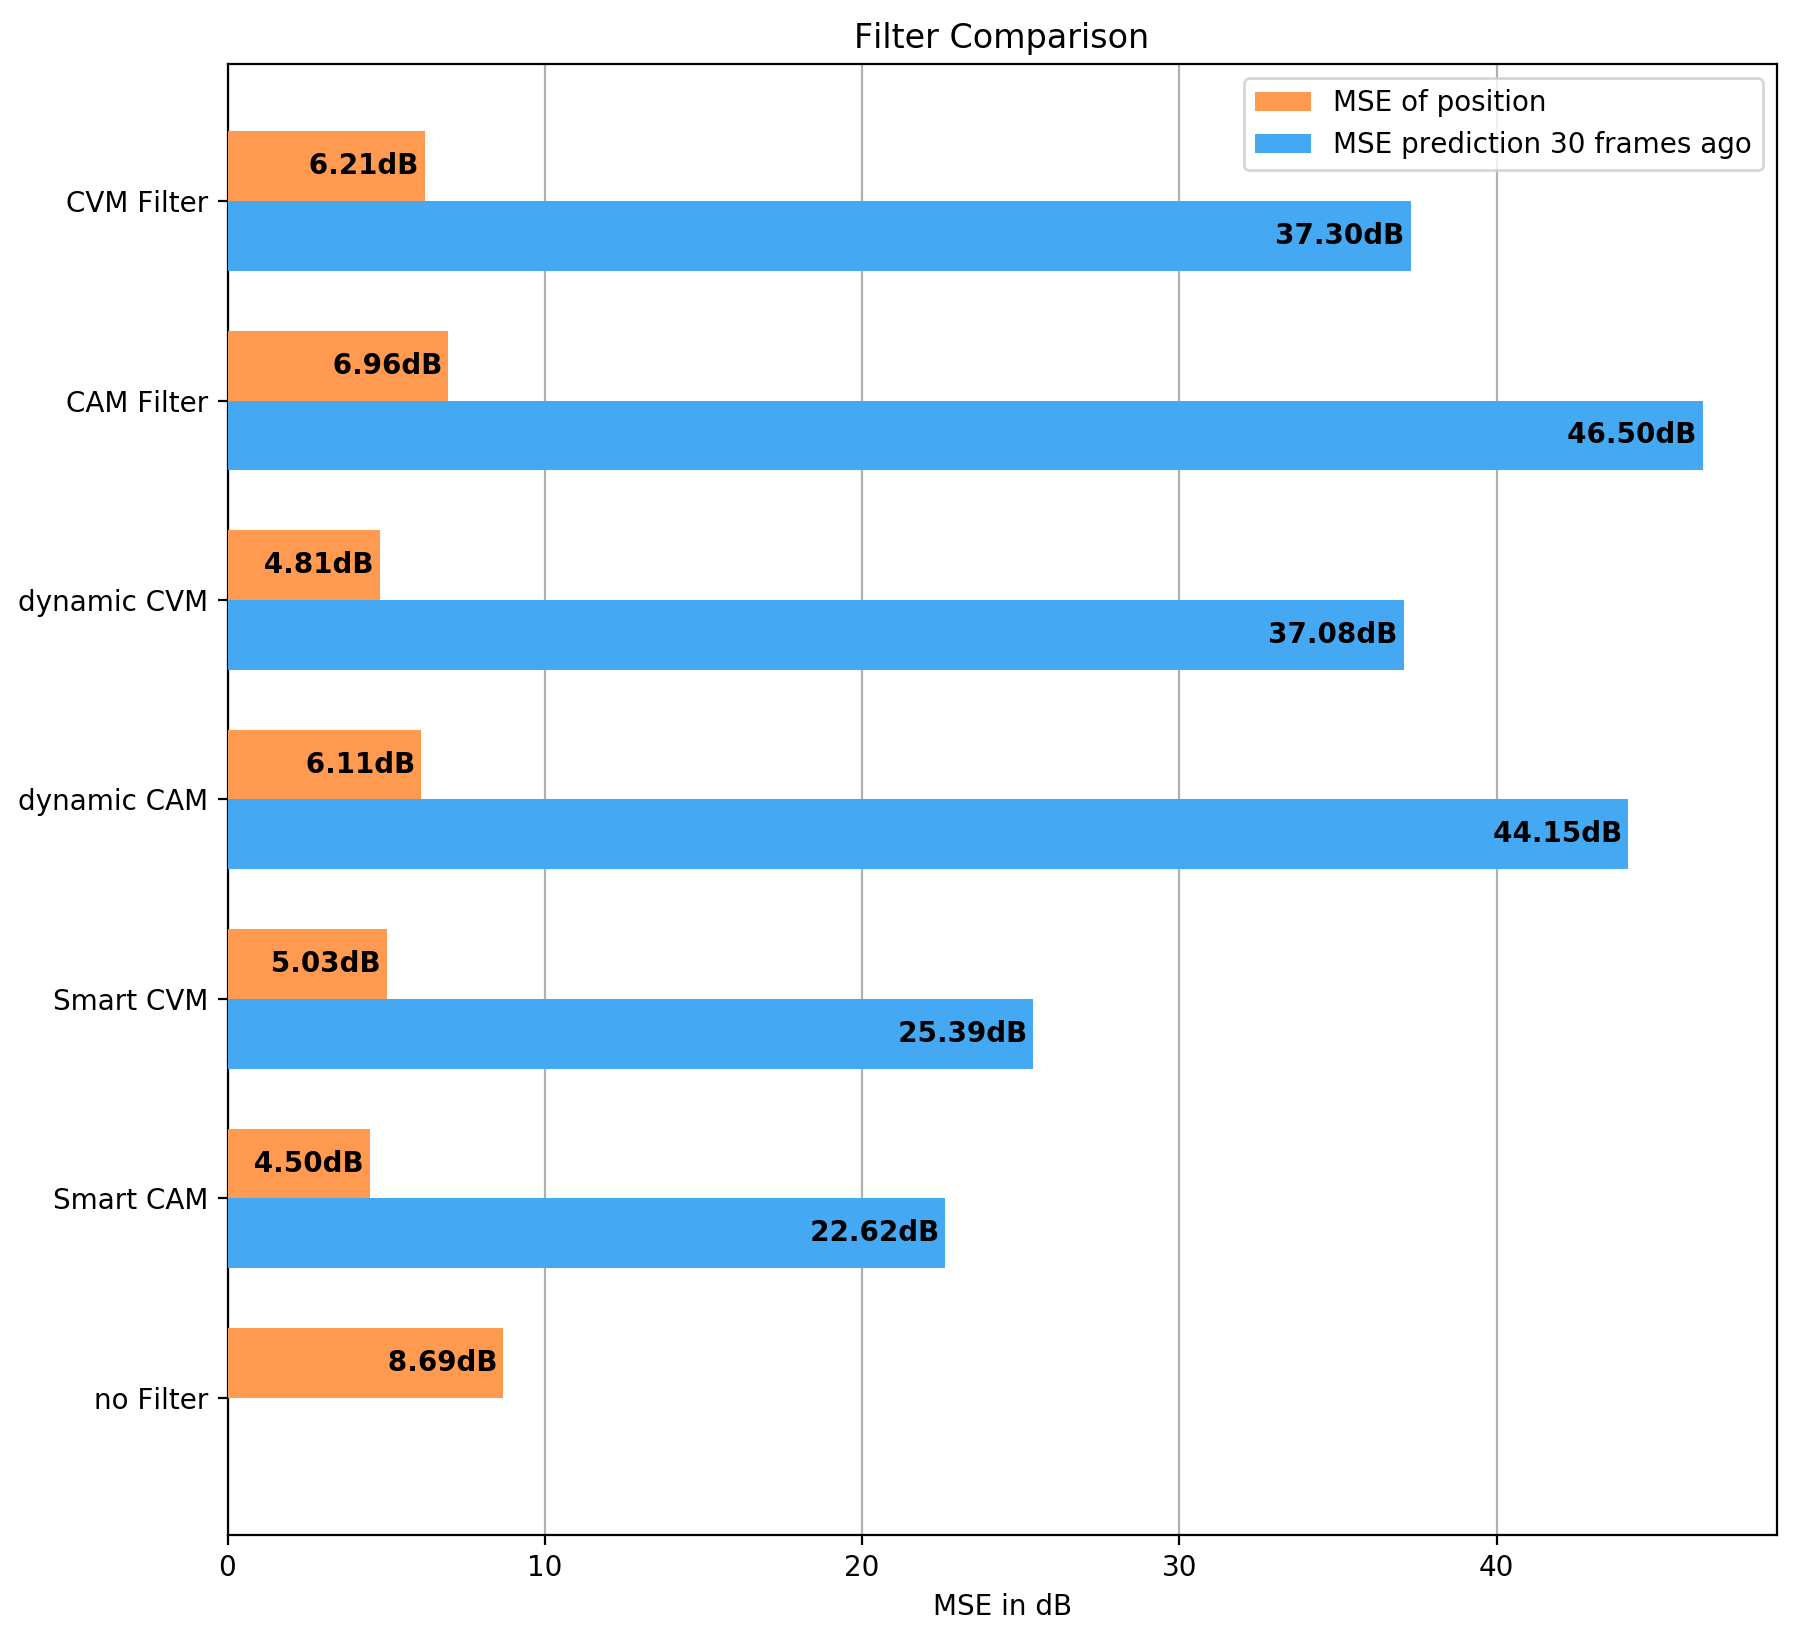
\includegraphics[width=0.47\textwidth]{filter_comparison_horizontal.PNG}}
        \caption{Performance of different filter implementations}
        \label{fig:sim-results}
    \end{figure}


    \bibliography{updatedReferences} 
    \bibliographystyle{ieeetr}


\end{document}